\documentclass[preprint,12pt,authoryear]{elsarticle}

\usepackage[utf8]{inputenc}

% Bibliograpy
\usepackage{natbib}
\usepackage{url}

% Acronyms
\usepackage{acro}

% Symbols
\usepackage{gensymb}
\usepackage{amsmath}

% Positioning
\usepackage{float}

% Colors
\usepackage[dvipsnames]{xcolor}

% Flowchart
\usepackage{tikz}
\usetikzlibrary{shapes,positioning,calc}

% Graphs
\usepackage{pgfplots}
\usepackage{pgfplotstable}
\usepgfplotslibrary{external}
\pgfplotsset{width=1\textwidth,height=0.7\textwidth,compat=1.9}

\usepackage{graphicx}
\graphicspath{ {./images/} }

\usepackage{subcaption}

% Links
\usepackage[linktoc=all]{hyperref}
\hypersetup{
	pdftitle={Development of a Finger-Key Identification Module for a Touch Typing Trainer},
	pdfstartview={FitH},
	colorlinks=true,
	linkcolor=black,
	citecolor=black,
	filecolor=black,
	urlcolor=MidnightBlue
}

% Tables
\usepackage{booktabs}
\usepackage{array}
\newcolumntype{P}[1]{>{\centering\arraybackslash}p{#1}}
\newcolumntype{R}[1]{>{\raggedleft\let\newline\\\arraybackslash\hspace{0pt}}m{#1}}


\DeclareAcronym{iso}{
	short=ISO,
	long=International Organization for Standardization
}


\DeclareAcronym{ansi}{
	short=ANSI,
	long=American National Standards Institute
}

\DeclareAcronym{jis}{
	short=JIS,
	long=Japanese International Standards
}

\DeclareAcronym{wpm}{
	short=WPM,
	long=Words per Minute
}

\DeclareAcronym{neck}{
	short=WRNULD,
	long=Work-related neck and upper limb disorders
}

\DeclareAcronym{cv}{
	short=CV,
	long=Computer Vision
}

\DeclareAcronym{roi}{
	short=ROI,
	long=Region of Interest,
	long-plural-form=Regions of Interest
}

\DeclareAcronym{cts}{
	short=CTS,
	long=Carpal Tunnel Syndrome
}

\DeclareAcronym{jwt}{
	short=JWT,
	long=JSON Web Tokens
}

\DeclareAcronym{fpacc}{
	short=FP ACC,
	long=Finger Placement Accuracy
}

\DeclareAcronym{hfpacc}{
	short=HFP ACC,
	long=Historical Finger Placement Accuracy
}

\DeclareAcronym{cps}{
	short=CPS,
	long=Characters per Second
}

\journal{International Journal of Human-Computer Studies}

\begin{document}

\begin{frontmatter}
	\title{Development of a Finger-Key Identification Module for a Touch Typing Trainer}
	\author[inst1]{Oscar Vian L. Valles}
	\ead{oscarvianvalles@gmail.com}
	\author[inst1]{Dhong Fhel K. Gom-os\corref{cor1}}
	\ead{dkgomos@up.edu.ph}
	\cortext[cor1]{Corresponding author at: Cebu City, Cebu, Philippines}
	\affiliation[inst1]{organization={Center for Research in Intelligent Systems, Department of Computer Science, University of the Philippines Cebu},
		country={Philippines}}


	\begin{abstract}
		Typing tests list out words for the user to repeat. These tests measure metrics
		that quantify the user's ability to type. However, conventional typing metrics
		do not measure correct finger placement. This aspect of typing may affect the
		user's health. It is also a crucial aspect of keyboard typing education. As
		such, a method to identify which finger is used to press which key is
		beneficial. This paper introduces a technique to achieve this by developing a
		finger-key identification module that utilizes computer vision algorithms to
		detect the keys in a keyboard, and a ready-made machine learning solution to
		track fingers while typing. This module was successful in finger-key
		identification with an accuracy of 99.58\% in a dataset of 942 keypresses. The
		module also had an average finger-key identification time of 0.083 seconds,
		which allows the module to perform real-time finger-key identification for
		typing speeds up to 143.040 Words per Minute which is well beyond the median
		typing speed of the population. Furthermore, two metrics for correct finger
		placement were defined and were implemented in a proof-of-concept trainer: (1)
		Finger Placement Accuracy which computes the number of keys pressed using the
		correct finger in a typing test sequence, and (2) Historical Finger Placement
		Accuracy which evaluates the user's ability to press a certain key with the
		correct finger over multiple typing test sequences.
	\end{abstract}

	\begin{highlights}
		\item Automated identification of what finger was used to press a key with
		an accuracy of 99.58\% in a dataset of 942 keypresses.
		\item Finger-key identifications take an average of 0.083 seconds. This
			allows for finger-key identification for typing speeds up to 143.040 Words
			per Minute
		\item Two metrics for correct finger placement were created: Finger
		Placement Accuracy and Historical Finger Placement Accuracy
	\end{highlights}

	\begin{keyword}
		touch typing \sep keyboard typing metrics \sep touch typing trainer \sep
		computer vision \sep finger tracking
	\end{keyword}

\end{frontmatter}

\section{Introduction}
There are a lot of educational typing tests available that help people learn
touch typing, including Monkeytype, TypeRacer, and Keybr. These typing tests
list out words that are then typed out. The entered keys are then compared to
check if the user has typed the expected letter \citep{bartnik2021}. At the end
of the test, the time taken is calculated, and certain metrics are given.
Examples of metrics include \ac{wpm} and Accuracy \citep{arif2009}. However,
this method of examination leaves out a crucial part of typing --— correct
finger placement.

There have been studies that show the effect of keyboard typing on the human
body. These studies have shown that keyboard typing affects our neck, shoulder,
upper limb, wrist, arms, and fingers \citep{szeto2005, baker2007digit}. In
addition, it has been shown that 22\% of computer users sustain musculoskeletal
disorders of the upper extremity. This includes the neck, shoulder, hands, and
wrists. \citep{gerr2002}

Incorrect placement of the fingers exacerbates these issues. These erroneous
finger placements may cause the following hand and wrist positions: ulnar
deviation, forearm pronation, and wrist extension \citep{serina1999}. These
three are hand and wrist positions that are common in all activities, however,
prolonged periods in these positions, such as in typing, may cause injuries such
as Carpal Tunnel Syndrom \citep{toosi2015} and musculoskeletal disorders of the
upper extremity (\citet{marklin1999} as cited in~\citet{baker2007}).

These issues can be prevented through keyboard typing education. Keyboard typing
has been a part of the curriculum for a long time \citep{hoot1986} and studies
have continued to this day to continue to optimize and improve methods of
teaching keyboard typing to students. By starting to teach touch typing to
students early, these students will develop the potential for higher-level
keyboard typing \citep{donica2018}.

There have been tools created to facilitate the teaching of touch typing.
Keyboarding without Tears is a web-based application and 36-week curriculum that
teaches students touch typing by following the three stages of Motor Learning
Theory \citep{kwt}. Monkeytype and TypeRacer are two keyboard typing test
websites where users type a predetermined phrase, quote, or random words, and
metrics are given after the test \citep{bartnik2021, typeracer}. Keybr is
similar to Monkeytype and Typerace, in that they also have the users type a
predetermined phrase, quote, or random words. However, this application guides
the user by using statistics to create typing lessons that are appropriate to
the current typing proficiency of the learner \citep{keybr}.

However, these typing tests only measure the ability to type the correct
character and do not check correct finger placement. While educators may be able
to weed out bad habits manually, it is impractical for them to check each
student individually.

While there have been other studies that utilize hand and finger tracking as
input methods. Examples include studies by \citet{dorf2001} which used finger
tracking as an input method in augmented environments, \citet{chiang2014} used a
Kinect to track fingers to play virtual instruments, and \citet{yousaf2014}
created a virtual keyboard that operates using finger tracking. However, these
studies used hand and finger tracking as an alternative input method, rather
than supplementing physical keyboard typing.

There is currently no solution to check for correct finger placement while
typing on a physical keyboard. Thus, there is a need for automatically
identifying which finger is used to press which key during typing --- hereby
defined as finger-key identification.

The paper aims to create a finger-key identification module that accurately
identifies what finger was used to press a key at a point in time to help
develop better typing habits and healthier typing ergonomics through the use of
computer vision algorithms. The paper also aims to create metrics to quantify
finger placement during the duration of keyboard typing.

\section{Algorithm}

\subsection{Setup}
\label{section:metho-setup}

The experimental setup and configuration controlled three key elements: the
camera, the keyboard, and the environment. The camera used was a Logitech C920.
It was placed directly above the keyboard and captured in 720p/30fps. The
keyboard used was a light-colored 60\% keyboard in a modified \ac{ansi} layout.
This type of keyboard only has the alphanumeric portion of a full-size keyboard.
The color of the surface the keyboard rested on was dark. The contrasting color
of the surface and the keyboard was chosen to improve the performance of the
algorithm in keyboard detection. The entire environment was evenly lit with a
6500k LED bulb rated at 9 watts outputting 700 lumens.

This setup was used to collect data points to measure the algorithm's ability to
perform finger-key identification in a controlled environment.


\subsection{Keyboard Detection and Key Mapping}
\label{section:metho-algo-keyboard}

A computer vision algorithm was created as a starting point for mapping the keys
of the keyboard within a video. OpenCV \citep{opencv} was used as the image
processing library for this step.

\subsubsection{Get Image Map}
The first portion of the algorithm creates an image map that is overlaid over
the detected edges of the keyboard. This image map subdivides the keyboard into
multiple \acp{roi} where each \ac{roi} represents a key.

To do so, the input frame from the camera was converted to an 8-bit grayscale
image. The frame was then denoised by using a bilateral filter. This filter
removes noise while maintaining the edges. A Sobel filter was then used for edge
detection \citep{sobel2014}. Thresholding was then performed using Otsu's
algorithm \citep{otsu} to reduce the bit-depth of the image from 8 to 1. This
reduction of bit depth improves the performance in finding contours. Contours
were found using the algorithm of \citet{contours}.

The detected contours were then simplified as the output of the algorithm
results in multiple points. To find the four points of the edges of the
keyboard, the contours were sorted and the largest one was selected. The
Douglas-Peucker algorithm for line simplification \citet{douglas-peucker} was
then performed to reduce the contour points to the minimum amount. The contour
points were then sorted clockwise, as the algorithm of \citet{contours} does not
guarantee the arrangement of the contour points. There is a need for the points
to be ordered clockwise since each point will be paired to the edges of the
image map, which were sorted in clockwise order.

The image map was then stretched over the keyboard by using a perspective warp,
where the four points of the edges of the keyboard were the end position of the
four points on the edges of the image map. Figure~\ref{fig:metho-image-map}
presents a grayscale frame and the resulting image map from that frame.

In ideal cases, the number of points would be four, with each point
corresponding to the edges of the keyboard. However, there were times when other
objects would be within the frame, or they intersected with the keyboard. This
would result in a contour that would be defined by more than four points ---
which caused the entire algorithm to fail.

\begin{figure}[h]
	\centering
	\begin{subfigure}{.50\textwidth}
		\centering
		\includegraphics[width=.995\linewidth]{grayscale.png}
		\caption{Input image that was converted to grayscale}
	\end{subfigure}%
	\begin{subfigure}{.50\textwidth}
		\centering
		\includegraphics[width=.995\linewidth]{transformed-image-map.png}
		\caption{Transformed image map}
	\end{subfigure}%
	\caption{First and last step of getting the image map}
	\label{fig:metho-image-map}
\end{figure}

\subsubsection{Get Key Contour Points}
The second portion of the algorithm pre-computes the contour points of each key
in the keyboard based on the generated virtual map and the Key-Color Values map.

The color that corresponds to each key in the virtual map is stored in the
Key-Color Value map. Each individual \ac{roi} was isolated using the color
values stored in the map. The simplified contours of each \ac{roi} were then
obtained using the same method in finding and simplifying the contour of the
keyboard.

During testing using training data, a lot of the failures in finger-key
identification were due to the tight fit of the contour to the key. The contour
on its own did not give enough buffer for the placement of the finger. This
buffer was needed as, in some instances, the finger used to press the key was
not exactly on top of the key, but rather to its side. In addition, it was also
observed that the finger tracking does not annotate the very edge of the
fingertip, but rather, it labels somewhere in the middle of the fingernail. The
algorithm accounts for this situation by adding a buffer. This was achieved by
scaling the contour points by seven pixels on each side.

After the contours of all \acp{roi} were obtained, a Key-Edge Coordinates map
was generated.


\subsection{Finger Detection and Tracking}
\label{section:metho-algo-finger}
MediaPipe Hands \citep{mediapipe} was used as the finger detection and tracking
solution. This algorithm is composed of two ML models working in conjunction to
be able to detect the different parts of the hands and track them accurately.
This algorithm outputs the positions of 21 hand and finger landmarks for each
hand within the image.

\subsection{Integration}

The two algorithms were combined to accomplish finger-key identification The
integration of the algorithm was a two-step process. The first step was to get
the Key-Edge Coordinates map shown in Section~\ref{section:metho-algo-keyboard}.
The second step runs whenever a key press has been detected. This step used the
Key-Edge Coordinates map in conjunction with the finger tracking algorithm
selected in Section~\ref{section:metho-algo-finger}.

The finger tracking data contained the pixel positions of each landmark of the
hands within the frame. The edge coordinates of the \ac{roi} of the key pressed
were obtained using the Key-Edge Coordinates map. Any fingertip landmarks that
fit within the \ac{roi} were then returned.

\section{Data Gathering}
Ten sentences were gathered from novels and texts in the public domain. These
sentences were used as typing test sequences. 3 sets of 10 videos were then
captured with each video corresponding to one typing test sequence. Each set
corresponds to three predetermined speeds of typing: slow (15wpm), average
(35wpm), and fast (80wpm). These speeds were based on test data
from~\citet{keybr}. Best effort was made to stick to the predetermined typing
speeds, however, there were discrepancies and the exact speed was not maintained
throughout the entire typing test sequence. During typing, errors were not
consciously taken into account, and errors happened naturally as part of the
typing process --- with more errors happening more frequently as the typing
speed increased.

Manual finger-key identification was performed for all key presses present in
the video. The annotated data was then divided into training and test data at a
ratio of 60:40, respectively.

\subsection{Data Inventory}

\begin{figure}[H]
	\begin{tikzpicture}
		\begin{axis}[
				xbar, xmin=0,
				bar width=3pt,
				width=0.9\textwidth,
				height=1\textwidth,
				enlarge y limits=0.02,
				xlabel=Count,
				symbolic y coords={
						Spacebar,
						Period,
						LeftShift,
						LeftAlt,
						ForwardSlash,
						Dash,
						Comma,
						Backspace,
						Z,
						Y,
						X,
						W,
						V,
						U,
						T,
						S,
						R,
						Q,
						P,
						O,
						N,
						M,
						L,
						K,
						J,
						I,
						H,
						G,
						F,
						E,
						D,
						C,
						B,
						A,
						1,
					},
				ytick=data,
				tick label style={font=\footnotesize},
				legend style={font=\footnotesize},
				label style={font=\footnotesize},
				xmajorgrids=true,
				area legend,
			]

			\addplot[
				CornflowerBlue,
				fill=CornflowerBlue
			] table[x=Value,y=Key]{test-data.txt};

			\addplot[
				Salmon,
				fill=Salmon,
			] table[x=Value,y=Key]{training-data.txt};
			\legend{Test Dataset, Training Dataset}
		\end{axis}
	\end{tikzpicture}
	\caption{Data Inventory}
	\label{fig:metho-inventory-training}
\end{figure}

Individual counts of the characters in the training and testing data set are
shown in Figure~\ref{fig:metho-inventory-training}. The letters were not
represented equally in the data set. Of note, J and Q were not in the training
dataset, and J, Q, and Z were not in the testing dataset. The inequality of
representation in both of these datasets can be attributed to the source
materials of the typing test sequences --- novels and texts. There was no
conscious decision to equally represent all characters in the data set.

\section{Training and Testing}
A script was created to test the accuracy of the module. This script opened each
video and the associated labeled file. There were three frames taken for each
video to perform step one of the module: frames ten, fifteen, and twenty. The
first frame that returned a Key-Edge Coordinates map was used. The script then
parsed the labeled file and opened the frame for each keypress. The second
algorithm of the module was then run. The result of the module was then compared
with the manual labeling of the keypress. Adjustments were then made to the
algorithm after each training pass to improve its performance.

The same script was run through the test data.

\section{Metrics}
\label{section:metric}

There were two total metrics obtained pertaining to finger and key mapping. The
first was per test sequence, and the second was per key.

\subsection{Per Test Sequence}
The metric which calculates per test sequence is \ac{fpacc}. This metric
computes the percentage of accurate keys pressed with the correct finger over
the length of the typing test sequence. Inputting the wrong character, even if
pressed with the correct finger, reduces \ac{fpacc} since \ac{fpacc} measures
\emph{accurate key presses}, and incorrect characters are considered inaccurate
key presses.

The equation for calculating \ac{fpacc} is as follows:

\begin{equation}
	FP ACC = \frac{|F|}{|T|} \cdot 100\%
\end{equation}


Where $|F|$ refers to the number of accurate keys pressed with the
correct finger and $|T|$ refers to the length of the text.

\subsection{Per Key}
This metric, \ac{hfpacc}, computes the accuracy of the user in pressing a
certain key with the correct finger over all test sequences. The same criteria
in determining accurate key presses. This allows the user to easily verify which
keys need attention and training if there is a high frequency of error.

The equation for calculating a key's \ac{hfpacc} is as follows:

\begin{equation}
	HFP ACC_{char} = \frac{|F_{char}|}{|C_{char}|} \cdot 100\%
\end{equation}

Where $|F_{char}|$ refers to the number of accurate keys pressed with the
correct finger for a certain character, identified as $char$. $|C_{char}|$
refers to the number of times the character has appeared in all test sequences
for the user.

\section{Proof of Concept Trainer}
A trainer was developed as a proof of concept of a real-world implementation of
the finger-key identification module. It consisted of three screens. The first
screen is where the keyboard was captured to perform get the Key-Edge
Coordinates map. The second screen is where the typing test is performed and
where real-time finger-key identification was done on each keypress. The third
screen shows the computed metrics as defined in Section~\ref{section:metric}. Of
note, the metrics shown on this page that uses multiple test sequences as an
input use tests that were obtained only during the current training session.
This proof of concept does not store the data of a user's previous test
sequences that were performed from a different session.

\section{Finger-Key Identification Accuracy}
Accuracy, in the context of the finger-key identification module, calculates the
percentage of successful finger-key identifications that the module has
performed. In this case, success is defined as having the expected finger, based
on the manual labeling, equal to the return value of the module. Accuracy is
calculated as:

\begin{equation}
	ACC = \frac{|S|}{|T|}
\end{equation}

Where $|S|$ is the number of successful finger-key identifications, and $|T|$ is
the total number of keypresses for all typing test sequences. This is also
referred to as the success percentage.

\subsection{Training Iterations}
There were a total of seven training iterations. These training iterations
served as a way to improve the performance of the module by adjusting its
parameters.

\subsubsection{Identifications}

\begin{figure}[H]
	\centering
	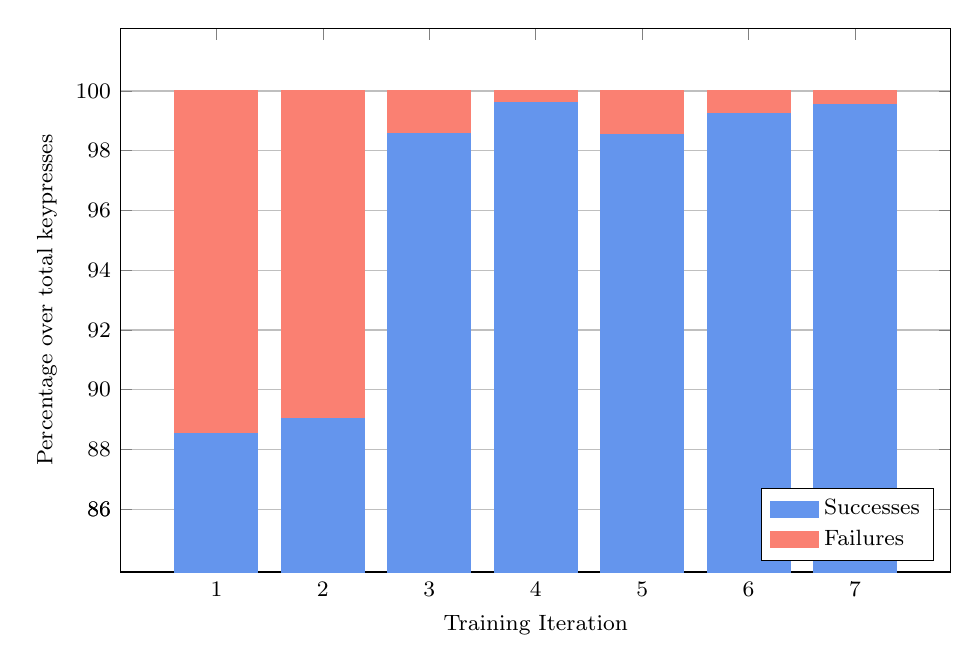
\begin{tikzpicture}
		\begin{axis}[
				ybar stacked,
				bar width=30pt,
				xlabel={Training Iteration},
				ylabel={Percentage over total keypresses},
				xmin=1, xmax=7,
				ymin=86, ymax=100,
				xtick={1,2,3,4,5,6,7},
				ytick={86, 86, 88, 90, 92, 94, 96, 98, 100},
				enlargelimits=0.15,
				area legend,
				tick label style={font=\footnotesize},
				legend style={font=\footnotesize},
				label style={font=\footnotesize},
				every axis legend/.append style={at={(0.98, 0.02)}, anchor=south east, cells={anchor=west}},
				ymajorgrids=true,
			]

			\addplot[
				CornflowerBlue,
				fill=CornflowerBlue,
			]
			coordinates {
					(1, 88.54) (2, 89.02) (3, 98.58) (4, 99.62) (5, 98.54) (6, 99.24) (7, 99.55)
				};
			\addplot[
				Salmon,
				fill=Salmon,
			]
			coordinates {
					(1, 11.46) (2, 10.98) (3, 1.42) (4, 0.38) (5, 1.46) (6, 0.76) (7, 0.45)
				};
			\legend{Successes, Failures}


		\end{axis}
	\end{tikzpicture}
	\caption{Identification results of the training iterations}
	\label{fig:rd-training-identification}
\end{figure}

Over the seven training iterations, there was an increase in success percentage
as shown in Figure~\ref{fig:rd-training-identification}. Consequently, there was
also a decrease in failure percentage. There was a total of 1475 total
keypresses for iterations one to three, and 1571 total keypresses for iterations
four to seven.

The increase in total keypresses starting from iteration four was due to adding
multiple tries to the training routine in obtaining the Key-Edge Coordinates
map. Iterations one through three only tried frame 10 as the source frame for
the module while iterations four through seven tried frames 10, 15, and 20.

There was a need to try different frames since the camera was not consistent in
its ability to focus on the keyboard for each video. In some videos video, the
camera was not focused on the keyboard in frame 10, but it was able to focus on
frame 15. As a result, the total number of available keypresses to test
increased.

The 0.48\% jump between iterations one and two can be attributed to correcting
erroneous finger-key identifications that were obtained from manual labeling.
The 9.56\% jump in success percentage between iterations two and three was due
to adding buffers around the \ac{roi} by scaling the contours by 10 pixels on
each side. Iteration four's increase was due to fixing the image map. Certain
keys had incorrect color values assigned in the Key-Color Values map, and some
keys were of incorrect shape. Iterations five to seven were performed to test
different values and shapes for scaling the \ac{roi}.

\subsubsection{Uncertain Successes}

\begin{figure}[H]
	\centering
	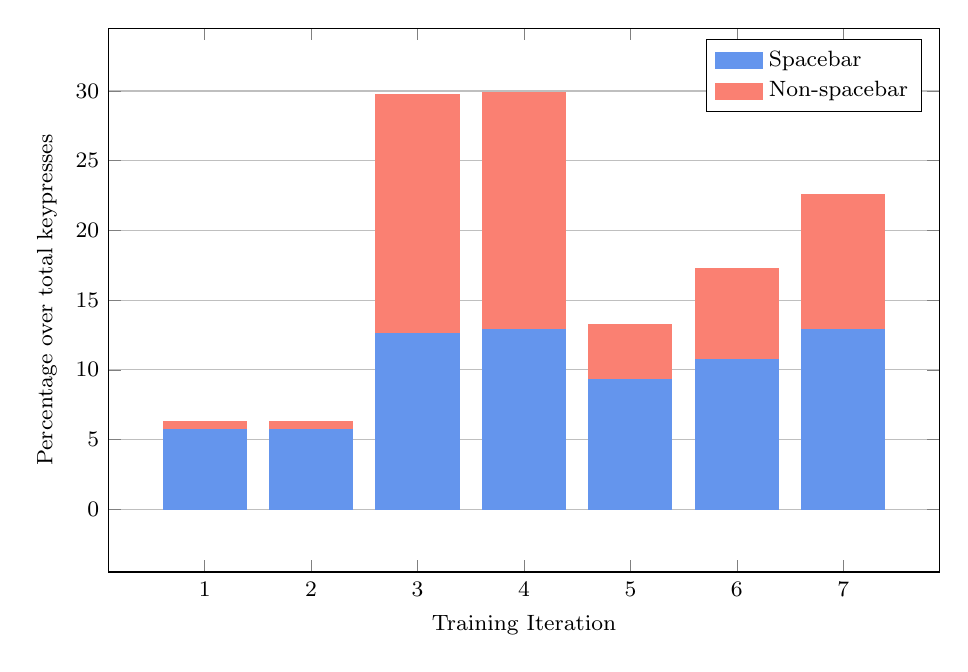
\begin{tikzpicture}
		\begin{axis}[
				ybar stacked,
				bar width=30pt,
				xlabel={Training Iteration},
				ylabel={Percentage over total keypresses},
				xmin=1, xmax=7,
				ymin=0, ymax=30,
				xtick={1,2,3,4,5,6,7},
				ytick={0,5,10,15,20,25,30},
				enlargelimits=0.15,
				area legend,
				tick label style={font=\footnotesize},
				legend style={font=\footnotesize},
				label style={font=\footnotesize},
				every axis legend/.append style={cells={anchor=west}},
				ymajorgrids=true,
			]

			\addplot[
				CornflowerBlue,
				fill=CornflowerBlue
			]
			coordinates {
					(1, 5.69) (2, 5.69) (3, 12.61) (4, 12.86) (5, 9.32) (6, 10.76) (7, 12.86)
				};
			\addplot[
				Salmon,
				fill=Salmon,
			]
			coordinates {
					(1, 0.61) (2, 0.61) (3, 17.15) (4, 17.06) (5, 3.95) (6, 6.49) (7, 9.68)
				};
			\legend{Spacebar, Non-spacebar}


		\end{axis}
	\end{tikzpicture}
	\caption{Uncertain Successes of the training iterations}
	\label{fig:rd-training-uncertain-successes}
\end{figure}

Uncertain Successes are instances where the finger-key identification module was
able to detect two or more fingertips within the \ac{roi} of the key. As such,
the module is uncertain which of the multiple fingertips pressed the key.
However, it is still classified as a success since the expected finger from the
manual labeling exists within the array of fingertips returned by the module.
Figure~\ref{fig:rd-training-uncertain-successes} shows the trend of this metric
throughout the different training iterations.

\paragraph{Spacebar}
In a 60\% keyboard, the spacebar is the longest key on the keyboard. In
addition, this key is right below the non-dominant hand's thumb's default
resting position when the hand's posture follows the proper touch typing
posture. As such, it was to be expected that a majority of the uncertain
successes were because of the spacebar. However, this was not the case for
iterations three and four. This was because the buffer for the \ac{roi} was too
big and this caused the module to detect more than one fingertip within that
\ac{roi}.

\paragraph{Non-spacebar}
There were cases where the module had uncertain successes that were not over the
spacebar. In almost practically all cases, these were over the alphanumeric
keys. These uncertain successes stem from the increased buffer of the \ac{roi}.
This type of uncertain success carries more weight compared to spacebar
uncertain successes since the keys where these uncertain successes come from are
the smallest keys on the keyboard. This means that the chances that a person has
two or more fingers over the keys are rare, compared to the spacebar.


\subsubsection{Uncertain Successes vs Success Percentage}
\label{section:rd-uncertain vs success}

\begin{figure}[H]
	\centering
	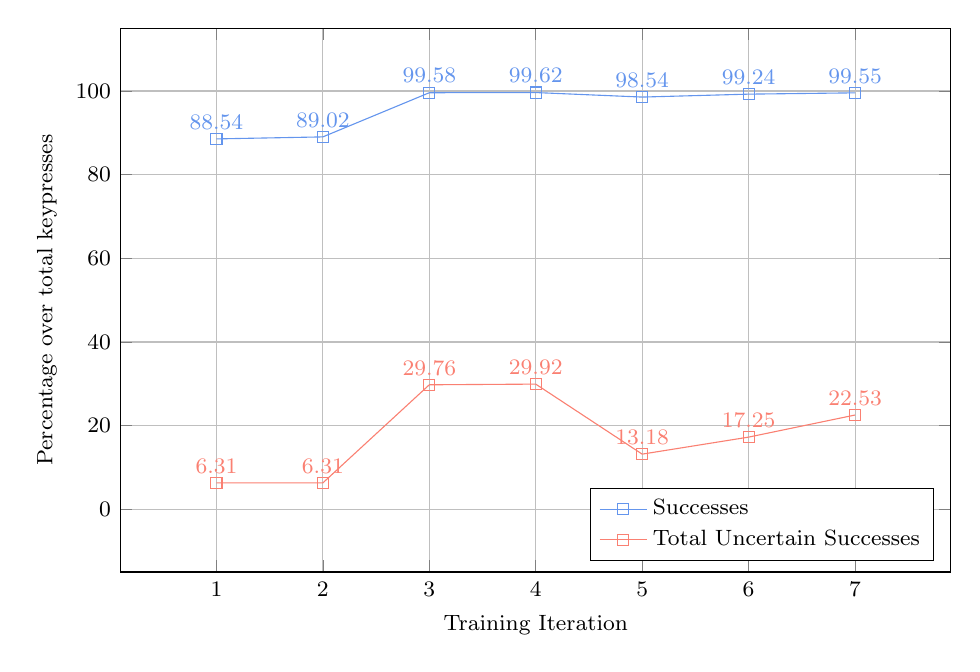
\begin{tikzpicture}
		\begin{axis}[
				xlabel={Training Iteration},
				ylabel={Percentage over total keypresses},
				xmin=1, xmax=7,
				ymin=0, ymax=100,
				xtick={1,2,3,4,5,6,7},
				ytick={0,20,40,60,80,100},
				tick label style={font=\footnotesize},
				legend style={font=\footnotesize},
				label style={font=\footnotesize},
				enlargelimits=0.15,
				ymajorgrids=true,
				xmajorgrids=true,
				nodes near coords,
				every node near coord/.append style={font=\footnotesize},
				every axis legend/.append style={at={(0.98, 0.02)}, anchor=south east, cells={anchor=west}}
			]

			\addplot[
				color=CornflowerBlue,
				mark=square,
			]
			coordinates {
					(1, 88.54) (2, 89.02) (3, 99.58) (4, 99.62) (5, 98.54) (6, 99.24) (7, 99.55)
				};
			\addplot[
				color=Salmon,
				mark=square,
			]
			coordinates {
					(1, 6.31) (2, 6.31) (3, 29.76) (4, 29.92) (5, 13.18) (6, 17.25) (7, 22.53)
				};

			\legend{Successes, Total Uncertain Successes}

		\end{axis}
	\end{tikzpicture}
	\caption{Uncertain Successes of the training iterations}
	\label{fig:rd-training-uncertain-successes-vs-success}
\end{figure}


Tuning the algorithm required managing both uncertain successes and the success
percentage and making compromises between one or the other. The goal of the
training process was to maximize the success percentage while limiting the
number of uncertain successes.

As seen in Figure~\ref{fig:rd-training-uncertain-successes-vs-success}, it can
be noted that in iterations one and two, the success rate was lower compared to
the other iterations. However, the percentage of uncertain successes was also
the lowest. Iteration three was the first iteration that created a buffer around
each key, however, this buffer of 10 pixels was too aggressive, with the
uncertain successes spiking upwards to nearly 30\%. Iteration five reduced the
buffer size by half to five pixels. This did not affect the success rate that
much, with only a reduction of 1.08\%. This also greatly decreased the uncertain
success percentage by 16.74\%. The sixth iteration met halfway between
iterations four and five, by adding a buffer of seven pixels. This increased the
success rate back to 99.24\% without greatly increasing the number of uncertain
successes. In comparison with the fourth iteration, the sixth iteration had its
success rate decrease by 0.38\%, but its percentage of uncertain successes
decreased by 12.67\%. A seventh iteration was trialed where the increase in
buffer was asymmetrical. For each key, the points nearer the user were increased
by 10 pixels, while the points farther away were increased by five pixels only.
This slightly increased the success rate by 0.31\%. However, the percentage of
uncertain successes also increased by 5.28\%.

While the percentage of uncertain successes in iterations five through seven was
in the range of 13\% to 20\%, The majority of these uncertain successes were
spacebar uncertain successes, as shown in
Figure~\ref{fig:rd-training-uncertain-successes}.

Based on these results, the final selected parameters for the module were the
parameters set in iteration six, with the buffer set to seven pixels as it was a
good middle ground between success rate and uncertain successes.


\subsubsection{Failure Types}

\begin{figure}[H]
	\centering
	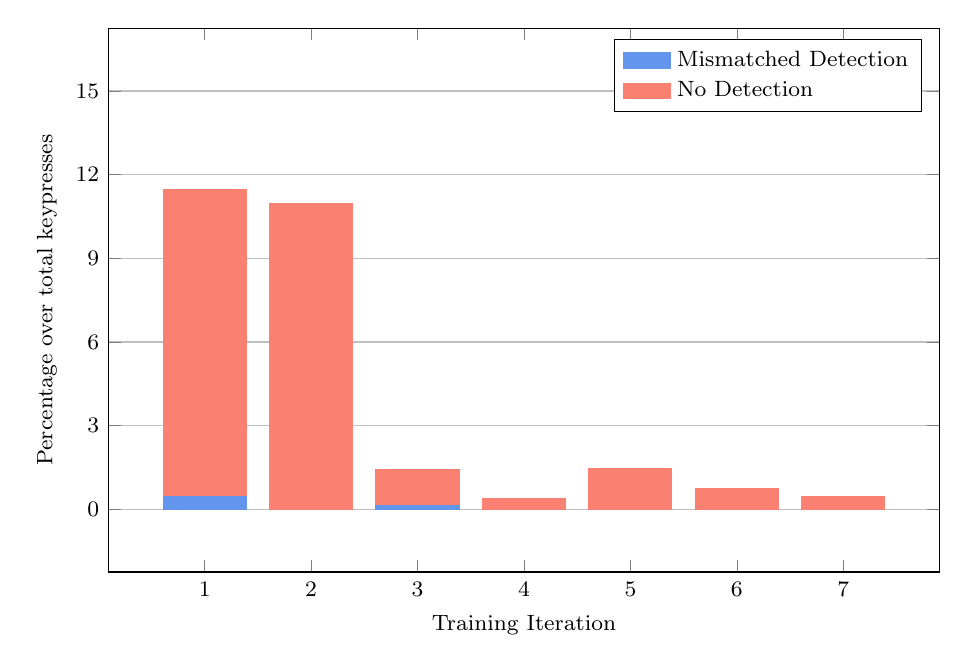
\begin{tikzpicture}
		\begin{axis}[
				ybar stacked,
				bar width=30pt,
				xlabel={Training Iteration},
				ylabel={Percentage over total keypresses},
				xmin=1, xmax=7,
				ymin=0, ymax=15,
				xtick={1,2,3,4,5,6,7},
				ytick={0,3,6,9,12,15},
				enlargelimits=0.15,
				area legend,
				tick label style={font=\footnotesize},
				legend style={font=\footnotesize},
				label style={font=\footnotesize},
				every axis legend/.append style={cells={anchor=west}},
				ymajorgrids=true,
			]

			\addplot[
				CornflowerBlue,
				fill=CornflowerBlue
			]
			coordinates {
					(1, 0.47) (2, 0) (3, 0.14) (4, 0) (5, 0) (6, 0) (7, 0)
				};
			\addplot[
				Salmon,
				fill=Salmon,
			]
			coordinates {
					(1, 10.98) (2, 10.98) (3, 1.29) (4, 0.38) (5, 1.46) (6, 0.76) (7, 0.45)
				};
			\legend{Mismatched Detection, No Detection}


		\end{axis}
	\end{tikzpicture}
	\caption{Uncertain Successes of the training iterations}
	\label{fig:rd-training-failure-types}
\end{figure}

\begin{figure}[h]
	\centering
	\begin{subfigure}{.33\textwidth}
		\centering
		\includegraphics[width=.995\linewidth]{failure-3.png}
	\end{subfigure}%
	\begin{subfigure}{.33\textwidth}
		\centering
		\includegraphics[width=.995\linewidth]{failure-1.png}
	\end{subfigure}%
	\begin{subfigure}{.33\textwidth}
		\centering
		\includegraphics[width=.995\linewidth]{failure-2.png}
	\end{subfigure}
	\caption{Example of No Identification Failures}
	\label{fig:rd-training-sample}
\end{figure}

\paragraph{Mismatched Identification}
These are failures where the module did not return the expected fingertip based
on the manual labeling. This type of failure only manifested in iterations one
and three. The failures in iteration one, after double-checking the video, were
due to an error during manual labeling. In iteration three, these errors were
due to an incorrect image map and Key-Color Values map. The information for some
keys was not consistent between both.

Based on this information and from the gathered data as shown in
Figure~\ref{fig:rd-training-failure-types}, this failure type is non-existent
for the module in real-life conditions.

\paragraph{No Identification}
These are failures where the module did not detect any fingertips within the
\ac{roi}. Figure~\ref{fig:rd-training-sample} shows examples of frames where
these errors occurred. These made up all the failures from the test results.
These types of failures occurred because the fingertips used to press the key
were not directly above the key, but rather offset to its side. Scaling the
\ac{roi} would reduce the number of no identification failures, but it would
also increase the number of uncertain successes. See
Section~\ref{section:rd-uncertain vs success} for more information.

\subsubsection{Occlusion}
The module was also successful in finger-key identification, even if both the
key and finger were occluded. Figure~\ref{fig:rd-occluded} is one frame where
this occurred. The module was successful in identifying that the Left Thumb was
used to press the Left Shift.

\begin{figure}[H]
	\centering
	\includegraphics[width=0.8\textwidth]{occluded.png}
	\caption{Occluded finger and key}
	\label{fig:rd-occluded}
\end{figure}


\subsection{Test Results}
\begin{table}[H]
	\small
	\centering
	\caption{\label{tab:rd-accuracy}Accuracy Results of the Module with Test Data}
	\begin{tabular}{ p{0.4\textwidth} R{0.2\textwidth} }
		\toprule
		Category                        & Value   \\
		\midrule
		Total Keypresses                & 942     \\[0.25cm]
		\midrule
		Identifications                           \\
		\midrule
		Successes                       & 938     \\
		Failures                        & 4       \\
		Success Percentage / Accuracy   & 99.58\% \\
		Failure Percentage              & 0.42\%  \\[0.25cm]
		\midrule
		Failure Types                             \\
		\midrule
		Mismatched Identification       & 0       \\
		No Identification               & 4       \\[0.25cm]
		\midrule
		Uncertain Successes                       \\
		\midrule
		Total                           & 133     \\
		Spacebar                        & 72      \\
		Spacebar Percentage             & 54.14\% \\
		Spacebar Percentage (Total)     & 7.64\%  \\
		Non-spacebar                    & 61      \\
		Non-spacebar Percentage         & 45.86\% \\
		Non-spacebar Percentage (Total) & 6.48\%  \\
		\bottomrule
	\end{tabular}
\end{table}

Table~\ref{tab:rd-accuracy} provides the accuracy results of the module with
test data. These results were satisfactory after running the module with the
parameters from the sixth training iteration on the test data. There was another
run with the same test data and the same parameters, however, these results were
omitted since this run had inconclusive results as there was a single
identification that was incorrectly labeled during manual finger-key
identification.

\section{Finger-Key Identification Speed}

\subsection{Training Iterations}

\begin{figure}[H]
	\centering
	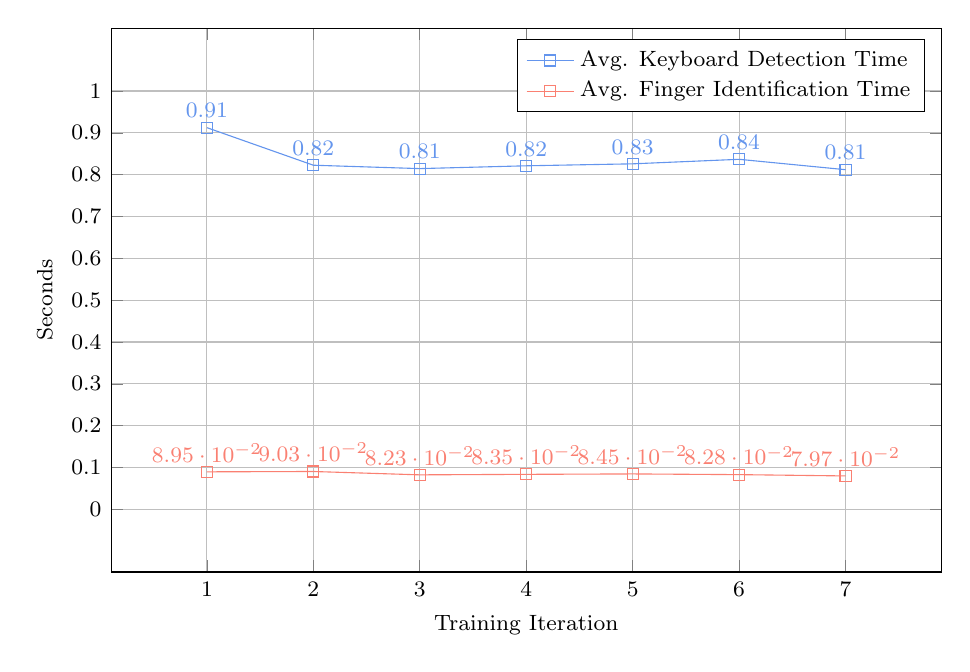
\begin{tikzpicture}
		\begin{axis}[
				xlabel={Training Iteration},
				ylabel={Seconds},
				xmin=1, xmax=7,
				ymin=0, ymax=1,
				xtick={1,2,3,4,5,6,7},
				ytick={0, 0.1, 0.2, 0.3, 0.4, 0.5, 0.6, 0.7, 0.8, 0.9, 1.0},
				tick label style={font=\footnotesize},
				legend style={font=\footnotesize},
				label style={font=\footnotesize},
				enlargelimits=0.15,
				ymajorgrids=true,
				xmajorgrids=true,
				nodes near coords,
				every node near coord/.append style={font=\footnotesize},
				every axis legend/.append style={cells={anchor=west}}
			]

			\addplot[
				color=CornflowerBlue,
				mark=square,
			]
			coordinates {
					(1, 0.9123) (2, 0.8225) (3, 0.8144) (4, 0.8211) (5, 0.8258) (6, 0.8366) (7, 0.8118)
				};
			\addplot[
				color=Salmon,
				mark=square,
			]
			coordinates {
					(1, 0.0895) (2, 0.0903) (3, 0.0823) (4, 0.0835) (5, 0.0845) (6, 0.0828) (7, 0.0797)

				};
			\legend{Avg. Keyboard Detection Time, Avg. Finger Identification Time}

		\end{axis}
	\end{tikzpicture}
	\caption{Keyboard detection time of the training iterations}
	\label{fig:rd-training-keyboard-detection-time}
\end{figure}

The training iterations had an average keyboard detection time of
$0.8620\pm0.0502s$ and an average finger identification time of
$0.0863\pm0.0040s$. Throughout the training, there was no noticeable difference
in running time over the same dataset as shown in
Figure~\ref{fig:rd-training-keyboard-detection-time}. However, the first
training iteration had issues with gathering the speed of the module, as the
average keyboard detection time included other operations that were not part of
getting the Key-Edge Coordinates map. Removing this iteration, the average
keyboard detection time becomes more consistent, with it being
$0.8295\pm0.0070s$.


\subsection{Average Keyboard Detection Time}
This is the time that was measured as the module generated the Key-Edge
Coordinates map. This corresponds with the first step of the module. It is to be
noted that this time does not affect keyboard typing and is not limited by the
0.32 threshold as the user is not yet typing at this point. The module got an
average keyboard detection time of 0.083s when ran on the test data.

\subsection{Average Finger Identification Time}
This is the time spent in finger-key identification for a single key. As such,
this time should be below 0.32 seconds for the module to be capable of
performing finger-key identification in real-time without noticeable slowdown
from the perspective of the user.

The average finger identification time that the module got when ran on the test
data was 0.083s which is well below 0.32s. This can be attributed to the speed
of the MediaPipe library, and the pre-calculation of the edge coordinates.

\subsubsection{Real-Time Finger-Key Identification}
Based on the definition of \ac{wpm} from \citet{arif2009}, it can be
extrapolated that calculating \ac{cps} is:

\begin{equation}
	CPS = \frac{WPM}{60} \cdot 5
	\label{eq:cps}
\end{equation}

The average \ac{wpm} when typing using the QWERTY layout, according to test data
from \citet{keybr} is $\approx37.5$ \ac{wpm}. As such, we can calculate
that the average Characters per Second when typing using the QWERTY layout is
3.125. We can calculate the seconds needed per character by this equation:

\begin{equation}
	s = \frac{1}{CPS}
	\label{eq:s}
\end{equation}

This means that each character, on average, requires 0.32 seconds to type. This
sets the maximum time spent for finger-key identification for a single
character. Any more than this would result in a noticeable slowdown during
typing.

With each keypress only requiring 0.083s for finger-key identification, it can
be gathered that the maximum \ac{cps} which the module can still perform
real-time finger-key identification is 11.9200 \ac{cps}, based on
Equation~\ref{eq:s}. It follows that the maximum \ac{wpm} that still allows for
real-time finger-key identification is 143.040 \ac{wpm}, based on
Equation~\ref{eq:cps}. This is well above the median of 37.5 \ac{wpm} on Keybr.
The module can also perform real-time finger-key identification for 90.99\% of the
community members of Monkeytype with the speed role.

\section{Conclusion}
The finger key identification module was successfully developed and implemented
in this study.

The finger-key identification solution was split into two parts, keyboard
detection and key mapping, and finger detection. Keyboard detection and key
mapping used the following algorithm and techniques: (1) Edge Detection using
Sobel filter \citep{sobel2014}, (2) Thresholding using Otsu's algorithm
\citep{otsu}, (3) Finding contours using the algorithm of \citet{contours}, (4)
line simplification using the Douglas-Peucker algorithm \citep{douglas-peucker},
and (5) Perspective transform \citep{opencv-docs}. Finger detection utilized a
ready-made solution called MediaPipe Hands by \citet{mediapipe}. The two were
combined to perform finger-key identification.

The keyboard used was a 60\% keyboard in ANSI. It was light in color and was
connected with a black USB-C cable. The surface of the desk was dark, and a LED
Bulb rated at 9 Watts, 700 lumens, and 6500k color temperature was used to
uniformly light the capture area. The single optical camera, a Logitech C920,
was placed above the keyboard, pointing directly downwards. It captured videos
in 720p/30fps with a diagonal field of view of 78\degree. The
computer used had an AMD Ryzen 5 3600 CPU, AMD Radeon RX 5600 XT GPU, G.Skill
Trident Z Neo RGB 16GB 3200mhz RAM, and Samsung SSD 850 EVO SSD.

The development of the module utilized OpenCV as the main image manipulation
platform that implemented the algorithms mentioned previously. OpenCV was also
used to capture videos from the optical camera. It was all written in Python.

The module was accurate in 99.58\% of identifications in a data set composed of
942 keypresses. However, 14.12\% of the identifications were uncertain
successes. These are successes where more than one fingertip was found in an
\ac{roi}. Of these, 6.48\% were non-spacebar uncertain successes. These are
uncertain successes over keys that are not the spacebar. This bears more weight
since most of these keys are the smallest on the keyboard, and in most cases,
only one fingertip could fit within the key. These uncertain successes were due
to the addition of a buffer around each \ac{roi} to increase the success rate.

The module is fast enough for real-time finger-key identification up to typing
speeds of 143.040 \ac{wpm}. This is above the median typing speed of 37.5
\ac{wpm} on Keybr \citep{keybr}. This also handles 90.99\% of the 12678 members
with the speed role on Monkeytype.

Two metrics were developed and implemented in a proof of concept trainer: (1)
Finger Placement Accuracy which computes the percentage of keys pressed with the
correct figure over the length of the test sequence, and (2) Historical Finger
Placement Accuracy which computes the number of times the user is successful if
pressing a key with the correct finger over all test sequences.

\section{Future Work}
There are a couple of ways to improve upon the module and its application. (1)
While a trainer was developed, this trainer is lacking in functionality to be a
usable trainer for teaching touch typing. (2) There were no tests done to prove
the effectiveness of the module on a learner's skill in touch typing, and there
was also no test done to prove that training using the module will improve
posture and reduce problematic hand positions and movements. (3) The
environmental setup was tightly controlled. This is not representative of
real-world conditions. (4) The keyboard used was specific. Supporting other
keyboard types, layouts, and color schemes would greatly increase the number of
users that could use the module. (5) The buffer of the \ac{roi} was selected
through trial and error. Adaptive techniques or machine learning algorithms
could select better values for the buffer. (6) The module is limited in its
ability to track keyboards that move between keypresses. (7) The dataset used
did not have an equal representation of all characters within the keyboard and
could be improved.

\section{CRediT authorship contribution statement}
\textbf{Oscar Vian L. Valles}: Conceptualization, Methodology, Software,
Investigation, Resources, Data Curation, Writing --- original draft, Writing ---
review \& editing, Visualization, Funding acquisition. \textbf{Dhong Fhel K.
	Gom-os}: Conceptualization, Methodology, Writing --- original draft, Writing
--- review \& editing, Supervision, Project administration

\section{Declaration of Competing Interest}
The authors declare that they have no known competing financial interests or
personal relationships that could have appeared to influence the work reported
in this paper.

\section{Acknowledgment}
We would like to recognize that this research was partially funded by the
Department of Science and Technology --- Science Education Institute

\bibliographystyle{elsarticle-harv}
\bibliography{references}

\newpage


\end{document}
